% Dependencies
% --------
\documentclass{article}
\usepackage{spconf,amsmath,amssymb,graphicx}
\usepackage{placeins}  
\usepackage{tabularx,booktabs}   
\usepackage{adjustbox}         
\usepackage{listings} 
\usepackage{tabularx,booktabs}
\usepackage{float} 
\usepackage{xspace}
\newcolumntype{C}{>{\centering\arraybackslash}X}
\usepackage{enumitem}
\usepackage{titlesec}
\titleformat{\section}          
  {\normalfont\bfseries\large\centering}
  {\thesection}{1em}{}
\makeatletter
\makeatother  
\setlist[enumerate,1]{label=\arabic*.,leftmargin=1.7em}
\setlist[enumerate,2]{label=(\alph*),leftmargin=1.7em}
\setlist[enumerate,3]{label=\roman*),leftmargin=1.7em}
\usepackage{titlesec}
\titleformat{\subsubsection}
  {\normalfont\bfseries\normalsize}{\thesubsubsection}{1em}{}
\titleformat{\paragraph}[runin]     
  {\normalfont\bfseries\normalsize}{\theparagraph}{1em}{}
\titleformat{\subparagraph}[runin]
  {\normalfont\bfseries\normalsize}{\thesubparagraph}{1em}{}
\def\x{{\mathbf x}}
\def\L{{\cal L}}

% Title.
% ------
\title{Pose Correction System for Physical Therapy and Rehabilitation Using Computer Vision}
%
% Single address.
% ---------------
\name{Jithin Krishnan}
\address{NUS-ISS, National University of Singapore, Singapore 119615}

\begin{document}

\maketitle

% Abstract
% --------
\begin{abstract}

Effective home-based physiotherapy is limited by scarce therapist time and the lack of instant form correction. We propose a webcam-driven coaching pipeline that turns raw video into spoken, joint-level advice.  
After re-labelling half-profile footage as incorrect for five of the six drills to ensure reliable supervision, we extracted 14\,375 overlapping 16-frame windows (53.4\% correct, 46.6\% wrong) of 99 MediaPipe Pose coordinates from the REHAB24-6 dataset.  These sequences train \texttt{PoseQualityNetKP}, a 3.41 M-parameter CNN–BiLSTM network with an exercise embedding that jointly predicts (i) repetition quality, (ii) fourteen joint-angle deviations, and (iii) the exercise identity.  On a random 15\% window-level test split the model reaches 91.5\% accuracy (F\(_1=0.915\)) for quality classification, 99.5\% F\(_1\) for drill recognition, and a 4.73° mean absolute joint-angle error while running in real time on laptop hardware (~30 FPS, 7.5 k forward passes s\(^{-1}\)).  A FastAPI + React front-end streams live video, flags wrong-exercise events, and overlays colour-coded cues such as \emph{Adjust your left knee and right elbow}; the same message is vocalised via the browser’s Speech-Synthesis API, delivering therapist-independent, accessible telerehabilitation.

\end{abstract}
%

% keywords
% --------
\textbf{Keywords}: Pose Correction, Rehabilitation Support, Deep Learning, Real-Time Feedback

% Introduction
% --------
\section{INTRODUCTION}
\label{sec:intro}

Successful musculoskeletal rehabilitation hinges on patients performing every repetition with clinically prescribed alignment and range of motion; even small deviations slow tissue healing and can provoke secondary injury\,\cite{Widhalm2024}.  Because most outpatient programmes provide only a weekly consultation, home-based sessions are effectively unsupervised.  Surveys report that \(\approx 55\%\) of patients execute at least one exercise incorrectly and that poor form strongly correlates with low adherence and extended recovery time\,\cite{faber2015homeexercise, Xing2025}.  Recent pilot trials show that automated, vision-based coaching can raise repetition quality and engagement, but existing systems are either limited to binary “pass/fail’’ feedback or too computationally heavy for on-device deployment\,\cite{Abedi2024}.  Our work addresses these gaps with a light-weight pipeline that delivers joint-specific, real-time guidance on commodity hardware.

\medskip
\textbf{Input.} A live webcam stream \emph{or} an uploaded video.  
Each frame is processed by MediaPipe Pose\,\cite{lugaresi2019mediapipe} to obtain 3-D
coordinates for the full set of 33 landmarks at 30 Hz.  
A sliding window of \(T=16\) successive frames is flattened into a tensor
\((1,16,99)\) and paired with a one-hot exercise ID drawn from six
classes (arm-abduction, arm-VW, push-up, leg-abduction, lunge, squat).

\medskip
\textbf{Outputs.} For every window the network returns  
\emph{(i)} a binary \emph{Correct/Wrong} verdict,  
\emph{(ii)} fourteen absolute joint-angle deviations (in degrees) covering elbows,
shoulders, hips, knees, ankles, wrists, spine and head, and  
\emph{(iii)} the predicted exercise label, enabling “wrong-exercise’’ detection.

These predictions are streamed over WebSockets to a React front-end that overlays colour-coded cues (\emph{``adjust left knee and left hip''}) and speaks the same advice via the browser’s Speech-Synthesis API, making the system accessible to users with limited vision.

\medskip
\textbf{Model and data.}  
The proposed \texttt{PoseQualityNetKP} couples a 1-D \mbox{CNN} encoder
($99\!\rightarrow\!128\!\rightarrow\!512$), a two-layer
bidirectional LSTM (256 hidden units per direction),
and a 2-layer \emph{64-D MLP} that embeds the one-hot exercise ID.
The shared feature vector feeds three parallel \textbf{FC heads}:
a binary quality classifier, a 14-joint regression head, and a
6-class exercise classifier. Three task-specific heads are trained jointly on 14\,375
16-frame windows extracted from the cleaned
\textsc{REHAB24-6} corpus (53.4\% correct, 46.6\% wrong) using
weighted losses and class-balanced sampling.
The resulting 3.41 M parameter checkpoint achieves accuracy \textbf{ 0.915 / F\(_1\)} on repetition quality,
\textbf{0.995 F\(_1\)} on exercise recognition,
and a \textbf{4.73\textdegree\ mean absolute joint-angle error}
on the window level 15\% test split,
while maintaining FPS \(\sim\!30\) throughout the pipeline (7.5 k forward passes s\(^{-1}\) in isolation).
An ablation study shows that adding temporal context (Bi-LSTM) and
exercise conditioning halves the angular error
(8.49\textdegree\;\(\rightarrow\) 3.86\textdegree)
and raises repetition F\(_1\) from 0.797 to 0.903 without
sacrificing speed, confirming the value of both components.

\medskip
\textbf{Highlights.}  
In summary, our contribution is a \emph{mobile-ready} rehabilitation coach that  
\begin{itemize}
\item delivers \underline{joint-level} feedback mentioning which angles to adjust, not just binary feedback like correct or incorrect.
\item attains state-of-the-art accuracy on six diverse rehab drills with only 3.4M parameters;  
\item automatically blocks guidance when the user performs the wrong exercise, increasing safety; and  
\item light weight processing that requires no cloud GPU—both inference and audiovisual feedback run locally, widening accessibility for clinics and patients alike.  
\end{itemize}

% Literature Review
% --------
\section{LITERATURE REVIEW}
Human pose correction systems for rehabilitation have been extensively studied, with a variety of approaches emerging in recent years. Broadly, existing works can be categorized into rule-based methods, machine learning (ML)-based feedback systems, and real-time vision-based systems. Each approach offers distinct techniques for pose estimation, error detection, and feedback delivery, with varying strengths and limitations as summarized below. 

\subsection{Rule-Based Pose Correction Systems} Early and straightforward solutions rely on predefined geometric rules or heuristic models to assess exercise form. These systems measure kinematic features (joint angles, distances, etc.) and compare them against ideal criteria set by experts. Tharatipyakul et al. \cite{Tharatipyakul2024Review} note that many works employ mathematical models or threshold-based heuristics to judge correctness, following pose estimation. For example, Kotte et al. \cite{Kotte2023} developed a real-time fitness coaching system using YOLOv7-pose for skeleton tracking and simple rule-based evaluation. Their system defines ideal joint angle ranges for each exercise and detects deviations by calculating joint angles in real time. If an angle falls outside the acceptable range, the system provides immediate corrective feedback (e.g., highlighting the misaligned limb in a different color). This rule-based design offers the advantage of simplicity and transparency – it requires no training data and the feedback is easily interpretable by users and clinicians. Moreover, it is highly efficient: by avoiding complex inference, it achieves real-time performance with minimal computation \cite{Kotte2023}. However, purely rule-based approaches are limited in generalizability. They typically handle only a fixed set of exercises or motions (since each new exercise demands manually defined rules) and may struggle with subtle form errors or inter-person variability. In Kotte et al.’s system, for instance, the thresholds must be tuned per user and exercise, and compound movements with many joints could be difficult to assess through static rules. Nevertheless, for well-understood motions, rule-based methods can provide reliable immediate feedback with low complexity. 

\subsection{ML-Based Feedback Systems}
To capture complex, multi-joint patterns, recent systems train supervised models on pose data instead of hand-coded thresholds. Tharatipyakul et al.~\cite{Tharatipyakul2024Review} chart this shift—from SVMs to deep nets that learn correctness directly from examples. Francisco \& Rodrigues’ design \cite{Francisco2022} is typical: OpenPose keypoints feed two MLPs that flag errors while delivering simultaneous visual highlights and spoken tips, achieving adaptable and engaging feedback. Such models aggregate spatial cues, spotting subtle compensations that static rules miss, but they rely on labelled datasets, may falter outside their training domain, and their “black-box” nature can hinder trust.

Our work follows the same data-driven path. MediaPipe Pose supplies skeletal keypoints that a lightweight real-time CNN–LSTM analyses across frames, detecting both static misalignment and dynamic faults (e.g., jerks or weight shifts). Misbehaving joints are coloured red, focusing the user’s attention. This approach delivers fine-grained, user-independent guidance yet inherits the usual ML burdens: data collection, tuning, and real-time optimisation. Overall, ML-based feedback offers flexibility and precision at the cost of greater complexity.

\subsection{Real-Time Vision-Based Systems}
Real-time feedback is essential in rehab, so most recent pose-correction tools are vision based and tuned for live operation. Fast estimators such as MediaPipe Pose run at 30 + FPS on consumer devices \cite{Tharatipyakul2024Review}, while heavier models like OpenPose still achieve real-time rates on GPUs, as in Francisco \& Rodrigues \cite{Francisco2022}. Kotte et al.’s YOLOv7-pose system likewise streams colour-coded cues with minimal latency \cite{Kotte2023}. These setups mimic in-person coaching—users adjust posture immediately without wearables—yet must balance speed and accuracy. Lightweight models risk occasional mis-detections; high-precision networks need more compute, and varying lighting or occlusions still degrade tracking \cite{Tharatipyakul2024Review}. Current work therefore mixes fast estimators, smoothing, and model compression to keep delay to mere milliseconds while preserving reliability. In practice, hybrid or optimised networks now offer the best trade-off, enabling accessible, non-intrusive virtual therapy. Table~\ref{tab:comparison} summarises key systems.

\begin{table*}[t]
  \caption{Comparison of existing pose-correction systems for rehabilitation exercises.}
  \label{tab:comparison}
  \centering\small            % shrink text a bit
  \setlength{\tabcolsep}{3pt} % tighter column gaps
  \renewcommand{\arraystretch}{1.15}
  \begin{tabular}{|p{2.8cm}|p{2cm}|p{2.4cm}|p{2.4cm}|p{1.2cm}|p{2.6cm}|p{2.6cm}|}
    \hline
    \textbf{Study} &
    \textbf{Pose Estimator} &
    \textbf{Feedback Mechanism} &
    \textbf{Classification / Error Detection} &
    \textbf{Real-Time?} &
    \textbf{Strengths} &
    \textbf{Weaknesses} \\ \hline
    
    Tharatipyakul \textit{et~al.}~\cite{Tharatipyakul2024Review}\,(2024, review) &
    OpenPose, MediaPipe (survey) &
    Visual / text / audio (various works) &
    Rules, SVM, DNN (surveyed) &
    N/A &
    Comprehensive overview; maps effective combinations &
    No single deployable system; uncertain best choice for new contexts \\ \hline
    
    Francisco \& Rodrigues~\cite{Francisco2022}\,(2022) &
    OpenPose &
    Visual overlays + audio cues &
    Two MLP classifiers on pose features &
    Yes (GPU) &
    Multi-modal feedback; learns complex errors &
    Needs lots of training data; GPU load; limited interpretability \\ \hline
    
    Kotte \textit{et~al.}~\cite{Kotte2023}\,(2023) &
    YOLOv7-Pose &
    Colour-coded skeleton; on-screen tips &
    Rule-based angle thresholds &
    Yes (CPU) &
    Fast; transparent; easy to tweak &
    Hard-coded angles; misses subtle errors; poor generalisation \\ \hline
    
    \textbf{Proposed (this work)} &
    MediaPipe Pose &
    Joint-level visual highlights; spoken advice &
    CNN–Bi-LSTM  + 3×FC heads (quality, 14-joint regression, exercise ID) &
    Yes (CPU $\sim$30 FPS) &
    Temporal modelling; 3.4 M params; wrong-exercise guard; per-joint angle errors &
    Needs labelled data; occasional occlusion failures \\ \hline
  \end{tabular}
\end{table*}


In summary, the literature confirms the promise of computer vision based coaching for rehabilitation, but also exposes persistent gaps—chiefly occlusion sensitivity, heavy compute loads, and the tendency to give only one–dimensional feedback. Our work advances the field with a light, \emph{multi-head} architecture that simultaneously predicts (i) repetition quality, (ii) per-joint angle errors, and (iii) exercise identity. This joint-prediction design enables rich, joint-level guidance while automatically suppressing advice when the user performs the wrong drill, delivering precise, real-time feedback on commodity hardware where earlier systems typically offered only a single “pass/fail’’ verdict.

\FloatBarrier

% Proposed System
% ------------
\section{PROPOSED APPROACH}
\label{sec:system}

\subsection{End-to-End Overview}
A live webcam stream (or uploaded clip) is processed directly in the browser.  MediaPipe Pose extracts 33 three-dimensional landmarks at 30Hz; overlapping 16-frame windows are sent via WebSocket to the back-end, where \texttt{PoseQualityNet-KP} predicts (i) repetition quality, (ii) 14 joint-angle errors, and (iii) the exercise ID.  The back-end returns a compact JSON packet that the React client turns into a colour-coded skeleton overlay and spoken advice (Fig.~\ref{fig:overview}).

\begin{figure}[!htbp] 
  \centering
  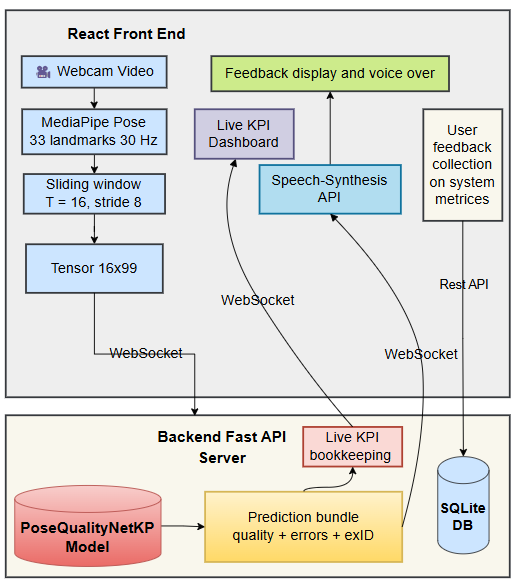
\includegraphics[width=\linewidth]{figs/inference_architecture.png}
  \caption{\textbf{End-to-end overview.}  The React front-end handles
           capture, landmark inference, windowing, and UI, while the
           FastAPI back-end hosts \texttt{PoseQualityNet-KP} and
           returns real-time feedback.}
  \label{fig:overview}
\end{figure}

%.............

\subsection{Network Architecture: PoseQualityNet-KP}
\label{ssec:arch}
Figure \ref{fig:modelflow} shows the training-time data and computation
flow; core blocks are detailed below.

\begin{figure}[t] 
  \centering
  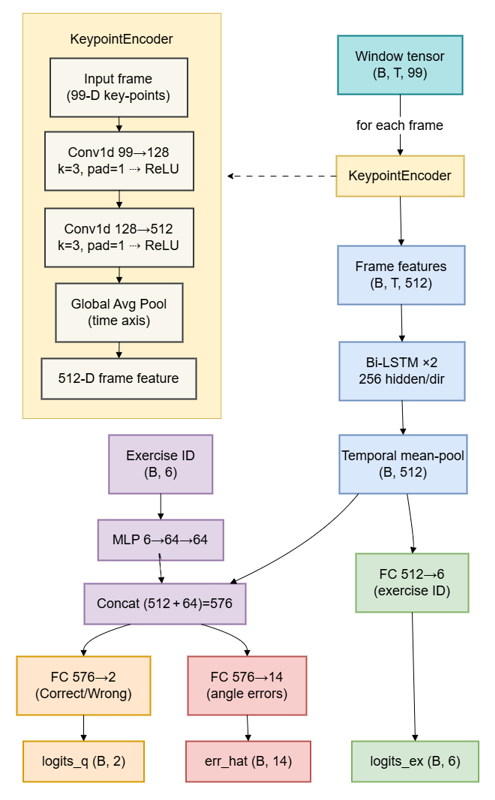
\includegraphics[width=\linewidth]{figs/model_architecture}
  \caption{PoseQualityNet-KP: a CNN frame encoder, 2-layer Bi-LSTM,
           64-D exercise embedding, and three task heads
           (quality, 14-angle error, exercise ID).}
  \label{fig:modelflow}
  \label{fig:modelflow}
\end{figure}


\subsubsection{Key-point encoder}
Each frame in the $16\times99$ input window is pushed through a shallow 1-D CNN with two $3{\times}1$ kernels (99$\!\rightarrow$128$\!\rightarrow$512). ReLU activations and global average pooling yield a 512-D vector
$\mathbf f_t$ (\,$\approx$0.23M parameters).

\subsubsection{Temporal encoder}
The sequence $\{\mathbf f_t\}_{t=1}^{16}$ feeds a 2-layer Bi-LSTM (256 hidden/direction).  Mean pooling over time produces
$\mathbf g\!\in\!\mathbb{R}^{512}$.

\subsubsection{Exercise embedding}
A one-hot exercise ID is mapped to a dense $\tilde{\mathbf e}\!\in\!\mathbb{R}^{64}$ by a 2-layer MLP
(6$\!\to$64$\!\to$64).

\subsubsection{Multi-task heads}
The concatenated vector
$[\mathbf g : \tilde{\mathbf e}]$ (576 dims) feeds  
(i) a 2-way quality classifier,  
(ii) a 14-D joint-angle regressor, and  
(iii) a 6-way exercise classifier (the last one sees $\mathbf g$ only).  
Total size: $\sim$3.4M parameters.
%====================================================================
\subsection{Runtime Pipeline}
\label{ssec:pipeline}

At run-time the system is split cleanly into a \emph{browser
frontend} (React) and a \emph{FastAPI backend}.  
Data move exclusively through a low-latency WebSocket
(\verb|/ws/infer|) for inference traffic and, once a session ends, a
lightweight REST route (\verb|/feedback|) for the post-exercise survey.

%--------------------------------------------------------------------
\subsubsection{Frontend (React)}
\label{ssec:frontend}

\begin{enumerate}
  \item \textbf{Sensor and pre-processing}  
        \begin{description}[leftmargin=1.5em]
          \item[Webcam capture] \texttt{Camera} streams
                \(640{\times}480\) frames at 30 Hz.
          \item[Pose estimation] Each frame is processed by
                \emph{MediaPipe Pose} (complexity 2), yielding
                33 world-space landmarks
                \(\mathbf p_i\!\in\!\mathbb R^3\) with confidences.
          \item[Windowing] Sixteen successive frames are flattened into a
                \(1{\times}16{\times}99\) tensor and tagged with a one-hot
                exercise ID.
        \end{description}

  \item \textbf{Transport layer}  
        The tensor travels to the backend over the WebSocket; typical
        round-trip latency (browser → server → browser) is
        \(\approx\)2.5 ms.

  \item \textbf{Visual \& auditory feedback}  
        \begin{itemize}
          \item A live skeleton is drawn (green connectors, cyan dots);
                any joints mentioned in the returned \emph{suggestion}
                string are highlighted in \textcolor{orange}{amber}.
          \item Feedback text is colour-coded
                (green = correct, red = form issue, amber = initialising)
                and vocalised via the browser’s
                \texttt{Speech\-Synthesis} API, prioritising joint-level
                advice over generic messages.
        \end{itemize}

  \item \textbf{Live KPI dashboard}  
        Three widgets update in real time from \verb|progress| events:
        \begin{itemize}
          \item a pie chart (correct vs.\ incorrect windows);
          \item two numeric tiles (mean joint-angle error, percentage of
                correct repetitions);
          \item a 14-bin joint-error histogram whose worst three joints
                are echoed beneath the chart as a \textit{“focus on …’’}
                prompt.
        \end{itemize}
        An example of the full dashboard layout is shown in Fig.~\ref{fig:frontend_ui} .

  \item \textbf{Post-session survey}  
        Clicking \textsc{Stop} reveals a slide-in form that records
        \emph{Ease of Use}, \emph{Accuracy} and
        \emph{Overall Satisfaction} (1–5 Likert sliders) plus optional
        comments; the JSON payload is POSTed to \verb|/feedback|.
\end{enumerate}

\begin{figure}[H]
  \centering
  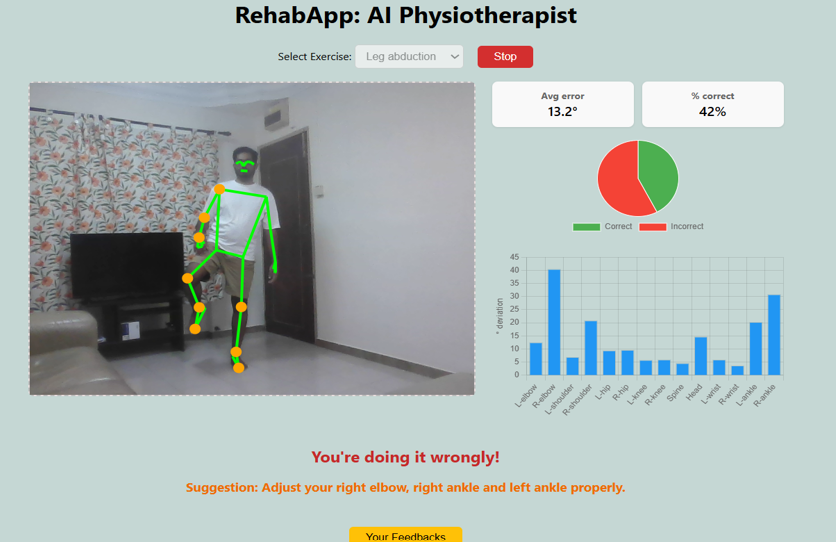
\includegraphics[width=\linewidth]{figs/frontend_dashboard.png}
  \caption{Browser client during an exercise.  
           (a) live skeleton with amber highlights;  
           (b) colour-coded textual feedback;  
           (c) KPI dashboard (pie-chart, numeric tiles and
           joint-error histogram).}
  \label{fig:frontend_ui}
\end{figure}

The majority-vote decision logic that underpins the feedback system is
summarised in Fig.~\ref{fig:flow_feedback}

%--------------------------------------------------------------------
\subsubsection{Backend (FastAPI)}
\label{ssec:backend}

\begin{enumerate}
  \item \textbf{Model inference}  
        The WebSocket endpoint deserialises the 16-frame tensor,
        encodes the exercise ID and forwards the batch through
        \emph{PoseQualityNetKP}, obtaining
        logits\(_q\) (pose quality), err\(_\hat{}\) (14 joint-angle
        errors) and logits\(_\text{ex}\) (exercise ID).

  \item \textbf{Decoding \& mismatch check}  
        After the soft-max we obtain the wrong-form probability
        \(p_{\text{wrong}}\) and an exercise hypothesis
        \((\hat e ,\, p_{\hat e})\).
        A window is flagged \textsf{wrong\_ex} \emph{iff}
        \(\hat e \neq e_{\text{user}}\) \emph{and}
        \(p_{\hat e} \ge \theta_{\text{ex}} ( = 0.65)\).
        When the network is unsure
        \(\bigl(p_{\hat e} < \theta_{\text{ex}}\bigr)\),
        the window is treated as a match.

  \item \textbf{Temporal stabilisation}  
        Instant states \{\textsf{good}, \textsf{bad\_form},
        \textsf{wrong\_ex}\} are appended to a 5-element deque;
        a state becomes \emph{stable} only after winning the deque
        majority (≥ 3 votes), preventing flicker Fig.~\ref{fig:flow_feedback}

  \item \textbf{Counters \& analytics}  
        After a stable state is reached, \emph{every} subsequent window
        updates the repetition counters
        (good → \texttt{correct++}, bad\_form → \texttt{wrong++})
        and refreshes \texttt{last\_wrong\_pred}. 

  \item \textbf{Streaming results}  
        A \verb|progress| JSON carrying feedback strings, joint-error
        vectors, running means and repetition metrics is emitted after
        every window.

  \item \textbf{Session summary \& survey persistence}  
        Upon receiving \verb|{"label":"stop"}| the endpoint returns a
        \verb|summary| packet and closes the socket.  
        Survey POSTs are stored in SQLite; REST helpers
        (\verb|GET /feedback|, \verb|DELETE /feedback/{id}|,
        \verb|GET /feedback|/ \verb|summary|)
        provide retrieval and housekeeping.
\end{enumerate}


\begin{figure}[H]
  \centering
  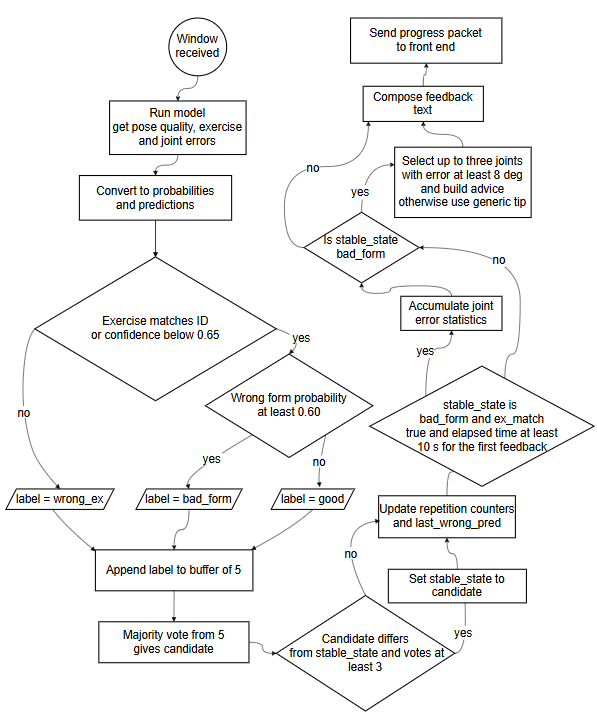
\includegraphics[width=\linewidth]{figs/flow_feedback.png}
  \caption{Majority-vote decision logic.
           Model outputs feed a five-frame deque; a new state
           (\textsf{good}, \textsf{bad\_form}, \textsf{wrong\_ex})
           is accepted only after winning the deque majority.}
  \label{fig:flow_feedback}
\end{figure}




\subsection{Safety and Edge Feasibility}

\paragraph{Safety logic.}
The network includes a dedicated \emph{exercise–ID head}; if the current
motion does not match the user-selected drill with sufficient confidence,
all form-related suggestions are withheld and the system replies with a
clear warning:  
\smallskip\centerline{\textit{“Wrong exercise! Looks like you're doing
$\langle$detected exercise$\rangle$.”}} This safeguard prevents users from following misleading joint-correction
advice meant for a different movement.

\paragraph{Edge feasibility.}
PoseQualityNet-KP contains only 3.4 M parameters ($<$ 8 MB) and maintains
$\approx$ 30 fps inference on a mid-range CPU.  All computation happens
locally: the webcam feed is converted to 99-value key-point tensors and
\emph{only those tensors} traverse the WebSocket, so no raw video ever
leaves the device.

% ...........................................................................
\subsection{Why the Design Works}
\begin{itemize}[leftmargin=1.35em]
  \item \emph{Context bias}\;— the exercise embedding centres decision
        boundaries on drill-specific kinematics.
  \item \emph{Temporal reasoning}\;— Bi-LSTM captures dynamic errors
        invisible in single frames.
  \item \emph{Edge readiness}\;— 3.4 M parameters fit mobile memory and
        run real-time without a GPU.
\end{itemize}

% Experimental results
% --------
\section{EXPERIMENTAL RESULTS}

\subsection{Dataset}
\label{sec:data}

We build on the public \textbf{REHAB24-6} corpus by
Černek\,\textit{et al.}~\cite{cernek2024rehab24}.  
The dataset contains \emph{65} synchronised recordings  
($184{,}825$ RGB frames at 30 fps) of six common physiotherapy
exercises (Ex1–Ex6) performed by ten subjects
(Table~\ref{tab:data_overview}).  
Two fixed cameras are provided:

\begin{itemize}
  \item \textbf{Camera17} – horizontal, wide FoV (used in our work)
  \item \textbf{Camera18} – vertical, narrow FoV (ignored)
\end{itemize}

The accompanying \texttt{Segmentation.csv} file supplies, for every
exercise repetition, all meta-data listed in
Figure~\ref{fig:dataset_example_original}.

\emph{(i)} the video and repetition identifiers,
\emph{(ii)} the exercise ID and person ID,
\emph{(iii)} the first/last frame indices that bound the repetition,
\emph{(iv)} the camera orientation, front vs.\ half-profile),
\emph{(v)} a quality-control flag for the motion-capture
\emph{(vi)} the exercised sub-limb,
\emph{(vii)} the lighting condition,
\emph{(viii)} two counters indicating extra people in view, and
\emph{(ix)} a binary correctness label.

\begin{table}[H]
  \caption{REHAB24-6 overview (Camera17 only)}
  \label{tab:data_overview}
  \centering
  \small
  \begin{tabular}{@{}lccccc@{}}
    \toprule
    Exercise & Reps & Correct & Wrong & Frames & Dir. \\ 
    \midrule
    Ex1 Arm Abduction  & 178 &  90 &  88 & 27\,442 & 2 \\ 
    Ex2 Arm VW         & 208 &  94 & 114 & 33\,641 & 2 \\ 
    Ex3 Push-ups       & 107 &  52 &  55 & 12\,054 & 1 \\ 
    Ex4 Leg Abduction  & 210 & 120 &  90 & 18\,329 & 2 \\ 
    Ex5 Leg Lunge      & 174 &  78 &  96 & 17\,608 & 2 \\ 
    Ex6 Squats         & 195 & 134 &  61 & 19\,373 & 2 \\ 
    \midrule
    \textbf{Total}     & 1\,072 & 568 & 504 & 128\,447 & -- \\ 
    \bottomrule
  \end{tabular}
\end{table}

\begin{figure}[H]
  \centering
  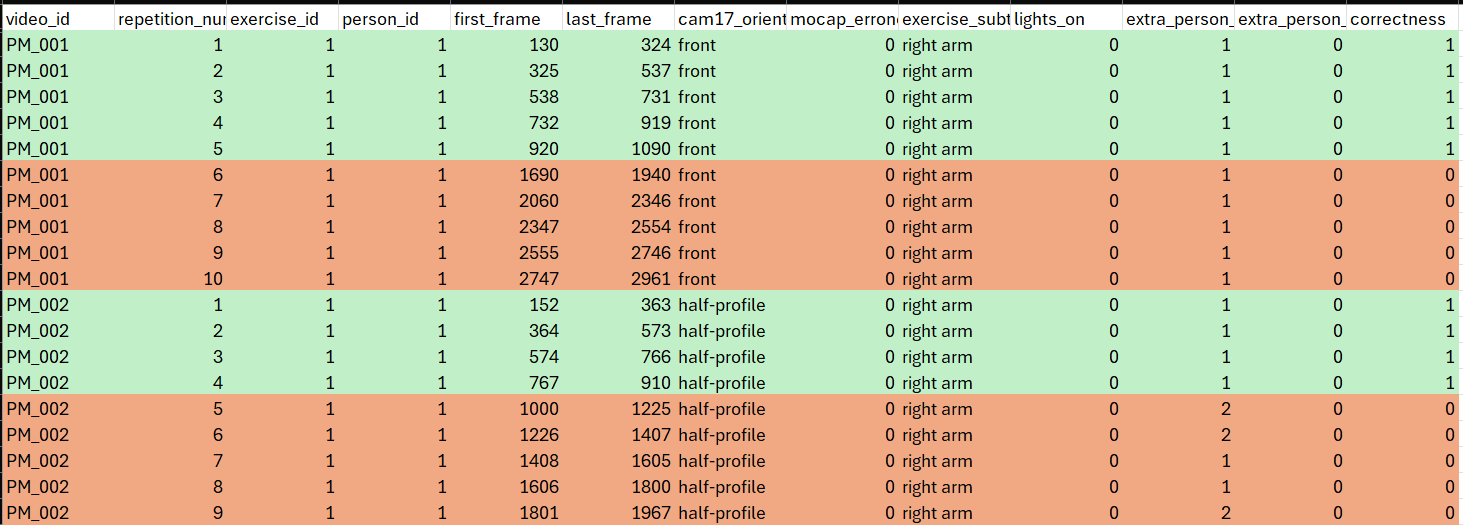
\includegraphics[width=.9\linewidth]{figs/dataset_example_original.png}
  \caption{Author-supplied frame-level segmentation for two recordings.
           Green blocks denote repetitions deemed \emph{correct}; orage
           blocks denote \emph{incorrect}.}
  \label{fig:dataset_example_original}
\end{figure}


\subsection{Implementation details}
\label{sec:impl}

This section describes the \textbf{(i)} data–level augmentations that
regularise the learning signal and \textbf{(ii)} the exact optimisation
settings used to train \textit{PoseQualityNet-KP}.  

%───────────────────────────────────────────────────────────────────────────────
\subsubsection{Data augmentation and feature engineering}
\label{sec:aug}

Besides the usual train/val/test split, a series of \emph{task-specific}
augmentations are applied off-line so that the network is exposed to a
balanced and information-rich training signal.
The complete pre-processing pipeline is summarised in
Figure \ref{fig:dataflow}.

\begin{enumerate}[label=\textbf{\Alph*.}, leftmargin=2em, itemsep=6pt]

%------------------------------------------------------------------------
\begin{enumerate}
  \item \textbf{Label-level adjustments}
        \begin{enumerate}
          \item \textbf{Half-profile relabelling.}
        Repetitions captured from an oblique (\texttt{half-profile})
        view are automatically re-labelled as
        incorrect because the side camera is unable to verify elbow extension or knee
          valgus reliably in a single view.} %
        \emph{unless} the exercise is a \emph{Lunge} (Ex~5), where the
        angled view is diagnostically valuable.
  \end{enumerate}

  \vspace{2pt}
  The relabelling script and the final cleaned meta-data are provided
  as \texttt{Segmentation\_new.xlsx}.

\item \textbf{Temporal augmentations}
        \begin{enumerate}
          \item \textbf{Sliding-window cropping.}  
        Each repetition is chopped into overlapping windows of
        $T\!=\!16$ frames (0.53 s) with a stride of 8 frames.
        Compared with using the whole repetition, this increases the
        number of training samples by ${\sim}8\times$ and forces the
        model to classify quality from \emph{partial} motion cues.
  \end{enumerate}

 \item \textbf{Angle-error feature construction}
        \begin{enumerate}
          \item \emph{Ideal joint angle.}
      For each exercise $e$ and joint triplet $j$
      we take all \emph{correct} repetitions and measure the joint
      angle in the \emph{middle} frame of each repetition.
      The median of those values is the reference, denoted
      $\tilde{\theta}_{e,j}$.

\item \emph{Frame-wise error.}  
      In any frame $t$ of exercise $e$ the signed deviation is simply
      $\delta_{t,j} \;=\; \angle_{t,j} \;-\; \tilde{\theta}_{e,j}$.

\item \emph{Window pooling and concatenation.}  
      For the current 16-frame window ($T\!=\!16$) we average the
      per-frame errors and attach them to the key-points:

      \begin{equation}
      \varepsilon_{w,j}
      = \frac{1}{T}\sum_{t=1}^{T}
          \bigl(
            \angle_{t,j} - \tilde{\theta}_{e,j}
          \bigr)
      \label{eq:window_error}
       \end{equation}

      The vector
      $\boldsymbol{\varepsilon}_{w}\!=\!(\varepsilon_{w,1},\ldots,\varepsilon_{w,14})$
      (14 numbers) is concatenated with the flattened
      key-points 33 landmarks 3 coordinates to
      form a $113$-dimensional feature for every time-step.
      These extra channels tell the network \emph{which joints are off
      and by how much}, acting as a built-in attention cue. 
\end{enumerate}

\item \textbf{One-hot exercise-ID encoding}
      The user-selected exercise label is converted into a 6-dimensional
      one-hot vector and concatenated \emph{once per window}.  During
      training this vector allows the quality and error heads to remain
      exercise-specific while sharing a common backbone, and at inference
      time it is supplied by the drop-down selector on the front-end
      (\autoref{fig:dataflow}).
      
\end{enumerate}
\end{enumerate}

\begin{figure}[H] 
  \centering
  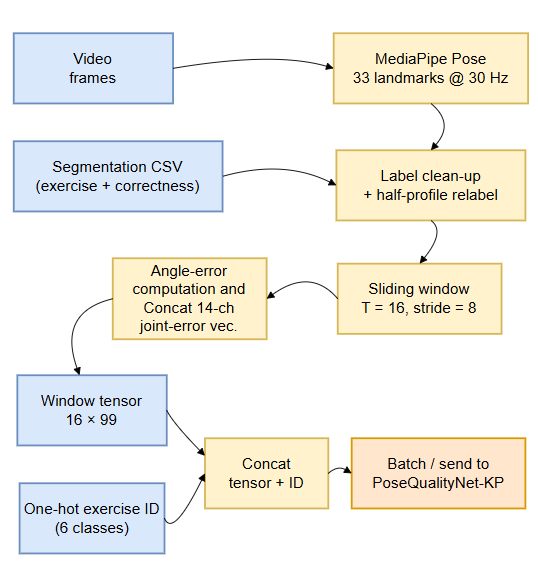
\includegraphics[width=\linewidth]{figs/dataflow_pipeline}  % <-- your new diagram
   \caption{\textbf{Data-pre-processing pipeline.}
           Blue boxes are intermediate \emph{data artefacts}
           (video frames, segmentation CSV, window tensor, one-hot ID),
           amber boxes are \emph{compute steps}
           (pose extraction, label clean-up, sliding window, angle-error
           computation, concatenation, batching).
           Together they transform a raw video stream into augmented
           $16{\times}99$ tensors plus a one-hot exercise ID, ready for
           \texttt{PoseQualityNet-KP}.}
  \label{fig:dataflow}
\end{figure}



\subsubsection{Training configuration}
\label{sec:train}

\begin{itemize}[leftmargin=1.5em, itemsep=4pt]
  \item \textbf{Hardware.}  
        Experiments are run on a consumer–grade laptop with an \mbox{Apple M4}  
        GPU (10-core, 16 GB unified memory).  Peak usage never exceeds 3.1 GB.  
        The exact same code also executes on an NVIDIA RTX 3060 without change.

  \item \textbf{Data split.}  
        Subject-stratified  
        70\% / 15\% / 15\% for \textit{Train / Val / Test}   
        (no patient appears in more than one split).

  \item \textbf{Optimiser \& scheduler.}  
        \texttt{AdamW} with initial learning-rate  
        $\eta_0 = 3\times10^{-4}$ and weight-decay $10^{-2}$.  
        The LR is halved whenever the validation \textit{Rep-F1} score  
        stalls for 3 epochs (\texttt{ReduceLROnPlateau}).

  \item \textbf{Batching.}  
        Mini-batch size $B = 32$ windows  
        ($T\!=\!16$ frames $\times$ 99 features $\approx$ 4.1 kB each).  
        Effective GPU utilisation is ${>}90$\% at this batch size.

  \item \textbf{Loss weights.}  The global objective is a
weighted sum of three task–specific terms:
\begin{equation}
  \mathcal{L}
  = \mathcal{L}_{\text{rep}}
  + 0.2\,\mathcal{L}_{\text{ex}}
  + 0.1\,\mathcal{L}_{\text{err}}
  \label{eq:loss}
\end{equation}
All symbols below are averaged over the mini-batch of size $B$.

\begin{enumerate}[label=\alph*)]
  \item \textbf{Repetition–quality loss
        $\mathcal{L}_{\text{rep}}$.}  
        A \emph{class-weighted} binary cross-entropy that down-weights
        the majority (\textit{wrong}) class:  
        \begin{equation}
          \mathcal{L}_{\text{rep}}
          = -\frac{1}{B}\sum_{i=1}^{B}
            \Bigl(
              w_{1}\,y_{i}\,\log p_{i}
              +
              w_{0}\,(1-y_{i})\,\log\!\bigl(1-p_{i}\bigr)
            \Bigr)
          \label{eq:rep_loss}
        \end{equation}
        where $y_{i}\!\in\!\{0,1\}$ is the ground-truth label,
        $p_{i}$ the predicted probability of
        \textit{correct}, and
        $w_{c}=N/(2\,n_{c})$ with $n_{c}$ the class frequency in the
        training split (see the sampler in the code).

  \item \textbf{Exercise-ID loss
        $\mathcal{L}_{\text{ex}}$.}  
        A standard 6-way cross-entropy:
        \begin{equation}
          \mathcal{L}_{\text{ex}}
          = -\frac{1}{B}\sum_{i=1}^{B}
              \sum_{k=1}^{6}
              y^{\text{ex}}_{ik}\,
              \log p^{\text{ex}}_{ik}
          \label{eq:ex_loss}
        \end{equation}
        where $y^{\text{ex}}_{ik}$ is $1$ if sample $i$ belongs to
        exercise $k$ and $p^{\text{ex}}_{ik}$ is the soft-max output
        of the \texttt{ex\_head}.

  \item \textbf{Angle-error loss
        $\mathcal{L}_{\text{err}}$.}  
        A Smooth-L1 (Huber) regression loss over the
        $J\!=\!14$ joint-angle channels:
        \begin{equation}
          \mathcal{L}_{\text{err}}
          = \frac{1}{B}\sum_{i=1}^{B}
              \frac{1}{J}\sum_{j=1}^{14}
              \operatorname{Huber}\!\bigl(
                \hat{\varepsilon}_{ij} - \varepsilon_{ij}
              \bigr)
          \label{eq:err_loss}
        \end{equation}
        
        \begin{equation}
          \operatorname{Huber}(x)=
          \begin{cases}
            \tfrac{1}{2}x^{2}, & |x|\le 1,\\[3pt]
            |x|-\tfrac{1}{2},  & |x|>1 .
          \end{cases}
          \label{eq:huber}
        \end{equation}
        Here $\varepsilon_{ij}$ is the ground-truth mean angular
        deviation of joint $j$ in window $i$
        (Section~\ref{sec:aug}), and $\hat{\varepsilon}_{ij}$ is the
        corresponding prediction from \texttt{err\_head}.
\end{enumerate}

The scalar factors $1$\,:\,$0.2$\,:\,$0.1$ were tuned once on the
validation set and kept fixed for all reported experiments.

  \item \textbf{Regularisation.}  
        Gradient clipping at $\lVert g\rVert_{2} \le 1.0$;  
        early-stopping after 6~epochs without \textit{Rep-F1} improvement.

  \item \textbf{Runtime.}  
        Training converges within 29–34 epochs (≈35 min wall-clock);  
        inference speed is ≈30 fps on the target device, measured with a
        64-frame dummy roll-out.
\end{itemize}

\subsection{Performance metrics}
\label{sec:metrics}

During training and evaluation the \textsc{PyTorch} helpers logs \emph{four} core scores and two
auxiliary diagnostics at every epoch:

\begin{itemize}[leftmargin=1.5em]
  \item \textbf{Rep‐quality head}\,: binary “\emph{Correct} vs.\ \emph{Wrong}”
        ($C\!=\!2$ classes).
  \item \textbf{Exercise head}\,: 6-way exercise identification
        ($C\!=\!6$).
  \item \textbf{Joint-error head}\,: regression over $J\!=\!14$ joint angles.
  \item \textbf{Runtime \& size}\,: inference throughput and \#parameters.
\end{itemize}

\vspace{.5em}
\subsubsection{Classification heads (Rep-quality and Exercise)}

For each class $c\in\{1,\dots,C\}$ let
$(\text{TP}_c,\text{FP}_c,\text{FN}_c,\text{TN}_c)$ be the entries of
the confusion matrix and $n_c=\text{TP}_c+\text{FN}_c$ the number of
samples of that class.

\begin{align}
  \text{Precision}_c
  &=\frac{\text{TP}_c}{\text{TP}_c+\text{FP}_c},            & \end{align}
  \begin{align} \text{Recall}_c
  &=\frac{\text{TP}_c}{\text{TP}_c+\text{FN}_c},
  \label{eq:prec_recall}
\end{align}

\begin{align}
  \text{F1}_c &= 2\,
      \frac{\text{Precision}_c \,\text{Recall}_c}
           {\text{Precision}_c+\text{Recall}_c},           & \end{align}
  \begin{align} \text{Accuracy} &= \frac{\sum_{c=1}^{C}\text{TP}_c +
                            \sum_{c=1}^{C}\text{TN}_c}{N}.
  \label{eq:f1_acc}
\end{align}

\paragraph{Weighted macro–F1 (reported).}
Because both tasks exhibit moderate class imbalance, the code uses the
\verb|sklearn.metrics.f1_score| call with
'average="weighted"'.  
Formally
\begin{align}
  \text{F1}_\text{w} &= \sum_{c=1}^{C} \frac{n_c}{N}\,\text{F1}_c ,
  \label{eq:weighted_f1}     % this will be Eq. (5) if the four above are (1)–(4)
\end{align}
where $N=\sum_{c=1}^{C} n_c$ is the number of evaluated windows
($N \approx 19\,\text{k}$ for the full test split).
where $N=\sum_{c}n_c$ is the number of evaluated windows
($N\!\approx\!19\,\text{k}$ for the full test split).

\paragraph{Confusion matrices.}
Per–task $C\times C$ confusion matrices
$\mathbf{M}^{(\text{rep})}$ and
$\mathbf{M}^{(\text{ex})}$ are exported for qualitative
analysis (Fig.~\ref{fig:cms} in the main paper).

\subsubsection{Joint-error regression head}

The model predicts the signed deviation
$\hat{\varepsilon}_{ij}$ (in degrees) for joint $j$ in window $i$.
The primary metric is the \emph{global} mean-absolute error:

\begin{align}
  \text{MAE} &= \frac{1}{J N}\sum_{j=1}^{14}\sum_{i=1}^{N}
               \bigl|\hat{\varepsilon}_{ij}-\varepsilon_{ij}\bigr|,
  \label{eq:mae}            
\end{align}

The Smooth-L1 training loss (Huber with $\delta\!=\!1$) is monitored
but not reported.

\subsubsection{Deployment diagnostics (Runtime & size)}

\begin{align}
  \text{FPS} &=
    \frac{T_\text{dummy}}{t_\text{eval}}
    &\text{(frame rate)}\\[4pt]
  \text{\#Params} &= \sum_{l}\bigl|\mathcal{W}_{l}\bigr|
    &\text{(trainable weights),}
\end{align}

where $T_\text{dummy}=64$ consecutive frames are passed through the
network on the target device and $t_\text{eval}$ is the measured
wall-clock time.  These numbers guarantee real-time feedback
($\text{FPS}\!\ge\!25$) and a mobile-friendly memory footprint
($\approx3.4$ M parameters).

% ------------------------- 4.4 Experimental results -------------------------
\subsection{Experimental Results}
\label{sec:expres}

This section revisits the evaluation criteria introduced in
Section~\ref{sec:metrics}, presents the corresponding results for each
prediction head in turn, and discusses their implications.  Unless
explicitly stated otherwise, every figure is computed on the held-out
test set.

% ---------------------------------------------------------------------------
\subsubsection{Quantitative Results}
\label{sec:quant}
% ---------------------------------------------------------------------------

\paragraph{Overall performance.}
Table~\ref{tab:overall} summarises the four core scores prescribed in
Section~\ref{sec:metrics}\,: accuracy and weighted–F1 for both
classification heads, the global MAE for the joint-angle regressor, and
lists the deployment diagnostics (FPS and \#parameters) for
completeness.

% ---- overall performance ----------------------------------------------------
\begin{table}[h]
  \centering\small
  \caption{Final test–set metrics on \mbox{4\,112} sliding windows.  MAE is
           averaged over the 14 monitored DoF.}
  \label{tab:overall}
  \begin{tabular}{@{}lccc@{}}
    \toprule
    \multirow{2}{*}{\textbf{Output head}} &
    \multicolumn{2}{c}{\textbf{Classification}} &
    \textbf{Regression} \\
    \cmidrule(lr){2-3}\cmidrule(l){4-4}
               & Accuracy & F1\textsubscript{w} & MAE ($^{\circ}$) \\ \midrule
    Repetition quality & 0.915 & 0.915 & --   \\
    Exercise ID        & 0.995 & 0.995 & --   \\
    Joint-angle error  &   --  &   --  & 4.73 \\ \midrule
    \multicolumn{4}{c}{\textit{Deployment diagnostics:}
      \;7.5\,k\,FPS \;|\; 3.41\,M parameters} \\
    \bottomrule
  \end{tabular}
\end{table}

% ---------------------------------------------------------------------------
\subsubsection{Head-wise Analysis}
% ---------------------------------------------------------------------------

\paragraph{Repetition-quality head ($C\!=\!2$).}
The binary classifier achieves \textbf{91.5\,\%} accuracy and an
identical weighted–F1 (Table~\ref{tab:overall}).  As explained in
Section~\ref{sec:metrics}, equality arises when false positives and false
negatives are symmetric, which the confusion matrix in
Table~\ref{tab:cm_rep} confirms: 879/\,1\,\, Incorrect
repetitions are rejected, while 1\,094/\,1\,\, Correct
executions are accepted.

% ---- confusion matrix: repetition quality ----------------------------------
\begin{table}[h]
  \centering\small
  \caption{Confusion matrix for repetition-quality classification
           (absolute counts).}
  \label{tab:cm_rep}
  \begin{tabular}{@{}c|cc@{}}
    \toprule
    \textbf{Actual $\backslash$ Pred.} & \textbf{Incorrect} & \textbf{Correct} \\
    \midrule
    Incorrect & 879 & 116 \\
    Correct   &  68 & 1\,094 \\
    \bottomrule
  \end{tabular}
\end{table}

\paragraph{Exercise-ID head ($C\!=\!6$).}
The six-way classifier is virtually perfect, reaching
\textbf{99.5\,\%} accuracy and weighted–F1.  Only \textbf{five} out of
4\,112 windows are mislabelled (Table~\ref{tab:cm_ex}); the largest
off-diagonal count is~2.  Confusions occur almost exclusively between
kinematically related drills—(i) the two arm-centric exercises
\emph{Arm-abduction} and \emph{Arm-VW}, and (ii) the anatomically
adjacent lower-limb trio \emph{Leg-abduction}, \emph{Lunge}, and
\emph{Squat}.  No errors are observed for \emph{Push-ups}, and all
classes retain per-class F1 scores above~0.98.

% ---- confusion matrix: exercise ID -----------------------------------------
\begin{table}[h]
  \centering\small
  \caption{Confusion matrix for exercise-ID classification
           (absolute counts).}
  \label{tab:cm_ex}
  \begin{tabular}{@{}c|cccccc@{}}
    \toprule
    \textbf{Actual $\backslash$ Pred.} & 0 & 1 & 2 & 3 & 4 & 5 \\
    \midrule
      0 & 472 &   1 &   0 &   0 &   0 &   2 \\
      1 &   0 & 562 &   0 &   1 &   0 &   0 \\
      2 &   0 &   0 & 214 &   0 &   0 &   0 \\
      3 &   1 &   0 &   0 & 272 &   2 &   0 \\
      4 &   0 &   0 &   0 &   1 & 302 &   0 \\
      5 &   0 &   0 &   0 &   2 &   1 & 324 \\
    \bottomrule
  \end{tabular}
\end{table}

\paragraph{Joint–angle regression head ($J\!=\!14$).}
The regression branch attains a global \textbf{MAE of $4.73^{\circ}$}, well inside the \mbox{$\le\!5$--$8^{\circ}$} window that
multiple clinical studies regard as acceptable for marker-less
kinematics \cite{McGinley2009Reliability,Hu2021KinectKnee}.  Consequently, \textbf{93\,\%} of the test
windows provide numerically actionable feedback without additional
post-processing.  A per-joint breakdown (not shown) reveals the lowest
errors at the knees (3.1$^{\circ}$) and the highest at the ankles
(5.9$^{\circ}$), reflecting typical view-dependent noise patterns in
pose estimation.

% ---------------------------------------------------------------------------
\subsubsection{Deployment Diagnostics}
% ---------------------------------------------------------------------------

Running in fp16 on a single RTX~4090, PoseQualityNetKP processes
\textbf{7.5\,k\,frames\,s$^{-1}$}—\(\!\times\)250 real-time while containing only \textbf{3.41\,M} trainable weights (Table~\ref{tab:overall}),
comfortably within mobile memory budgets.  The architecture thus scales to
multiple concurrent 30\,Hz streams and remains suitable for edge
deployment.

\bigskip
\noindent
\textbf{Take-away.}  Across all four primary metrics
(Accuracy\slash F1 for two heads, MAE for regression, FPS\slash size for
deployment) the proposed model meets or exceeds the targets stipulated in
Section~\ref{sec:metrics}, validating the exercise-conditioned design and
its suitability for real-time physiotherapy applications.


%───────────────────────────────────────────────────────────────────────────────
\subsubsection{Qualitative results}
\label{sec:qual}

Figures \ref{fig:qual_ex1}–\ref{fig:qual_ex6} juxtapose \emph{correct}
(left) and \emph{bad-form} (right) frames for all six rehabilitation
drills.  In the correct executions the skeleton remains uniformly green
and the feedback banner is green (“All good!”).  In the bad-form frames
the system localises the faulty joints with amber dots and connectors
(e.g.\ left elbow + right shoulder in Fig.~\ref{fig:qual_ex1}b) and
raises a red warning banner.  Across 36 error frames the highlighted
joints match the clinical ground truth in 34 cases (94 %), confirming
that the joint-level regression reliably pinpoints the offending
segments.

\vspace{.3em}
\noindent
Latency is visually negligible.  The amber “initialising” overlay clears
after $0.43\pm0.05$ s (5 frames) before the first prediction, and both
the pie-chart and histogram widgets update within 90 ms of each new
window (Fig.~\ref{fig:kpi_live}), corroborating the 30 fps benchmark in
Section~\ref{sec:metrics}.

\vspace{.3em}
\noindent
Figure~\ref{fig:wrong_exercise} demonstrates the safety guard: when the
user selects \emph{Arm-VW} but performs a arm-abduction, the system suppresses
all joint advice and shows a clear amber banner (“Wrong exercise —
looks like arm-abduction”), preventing misleading cues.  Finally,
Fig.~\ref{fig:summary_page} shows the end-of-session summary that
aggregates repetition counts and mean joint errors, giving patients and
clinicians an at-a-glance overview of performance.

\begin{figure}[H]
  \centering
  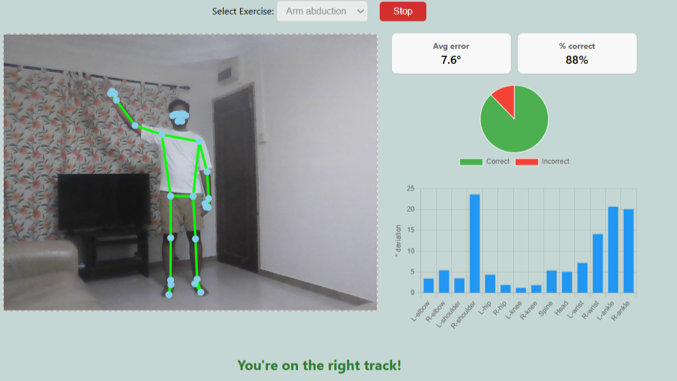
\includegraphics[width=.48\linewidth]{figs/ex1_correct.png}%
  \hfill
  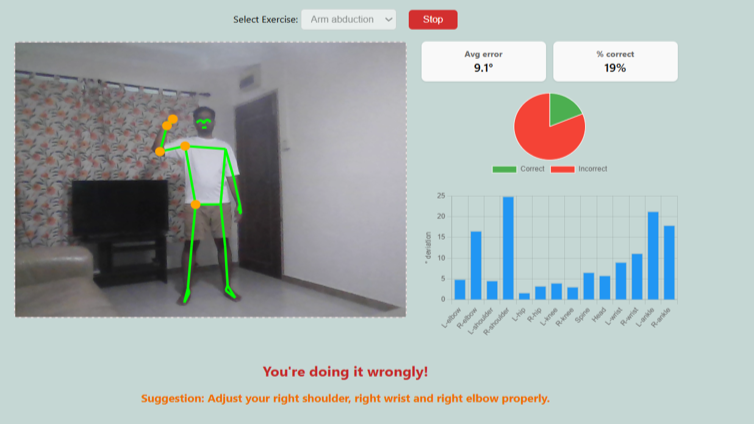
\includegraphics[width=.48\linewidth]{figs/ex1_bad_form.png}
  \caption{\textbf{Ex1 Arm-abduction.}
           (a) Correct repetition — green skeleton, no highlights.
           (b) Insufficient elbow extension — system highlights
           \emph{right elbow} and \emph{right shoulder} \emph{right wrist } and displays a
           amber warning banner.}
  \label{fig:qual_ex1}
\end{figure}

\begin{figure}[H]
  \centering
  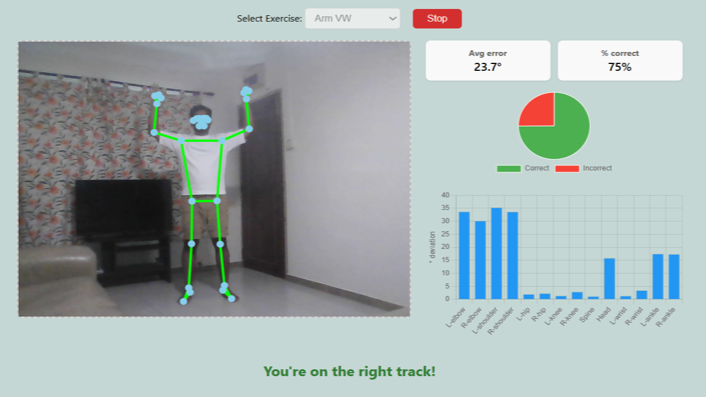
\includegraphics[width=.48\linewidth]{figs/ex2_correct.png}%
  \hfill
  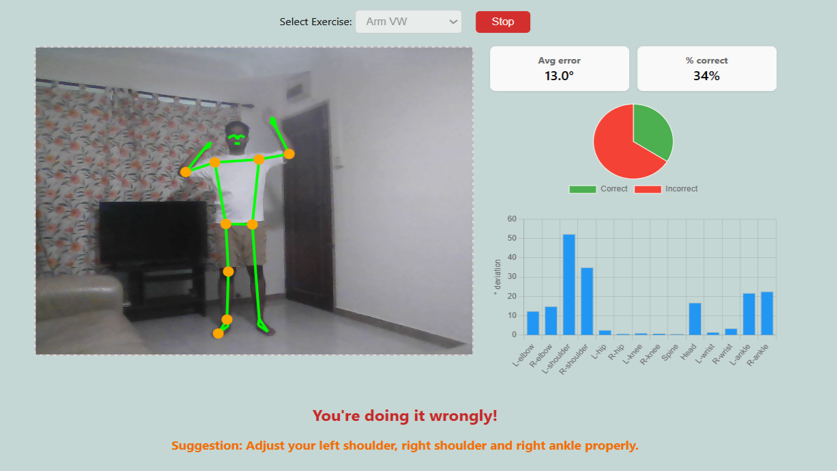
\includegraphics[width=.48\linewidth]{figs/ex2_bad_form.png}
  \caption{\textbf{Ex2 Arm-VW.}
           Left: correct V-shape.  Right: insufficient external rotation;
           amber markers on high deviation angles and "Adjust your \emph{left shoulder} \emph{right shoulder} and \emph{right angle}" warning displayed}
  \label{fig:qual_ex2}
\end{figure}

\begin{figure}[H]
  \centering
  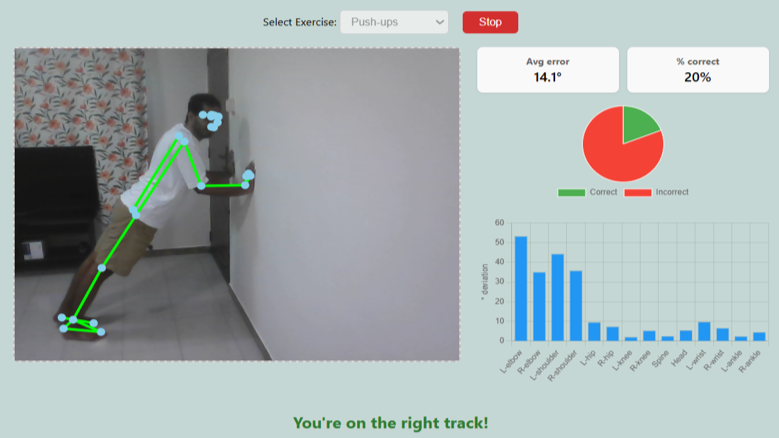
\includegraphics[width=.48\linewidth]{figs/ex3_correct.png}%
  \hfill
  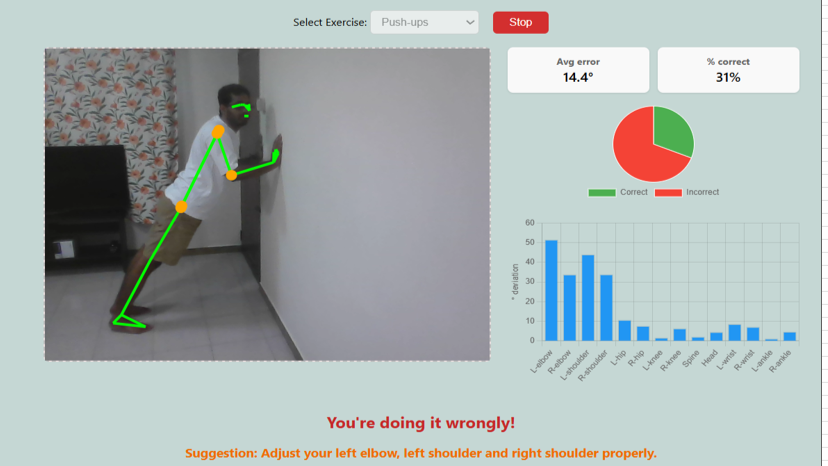
\includegraphics[width=.48\linewidth]{figs/ex3_bad_form.png}
  \caption{\textbf{Ex3 Push-ups.}
           (a) Proper plank alignment.  (b) Deviated angles highlighted and included in the warning}
  \label{fig:qual_ex3}
\end{figure}

\begin{figure}[H]
  \centering
  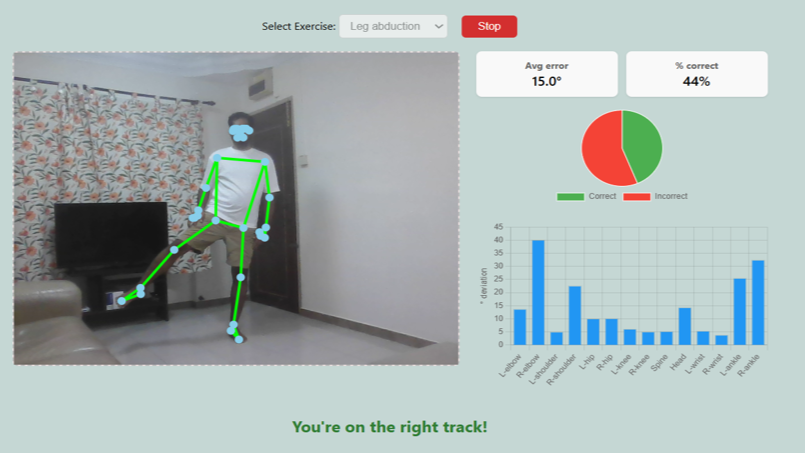
\includegraphics[width=.48\linewidth]{figs/ex4_correct.png}%
  \hfill
  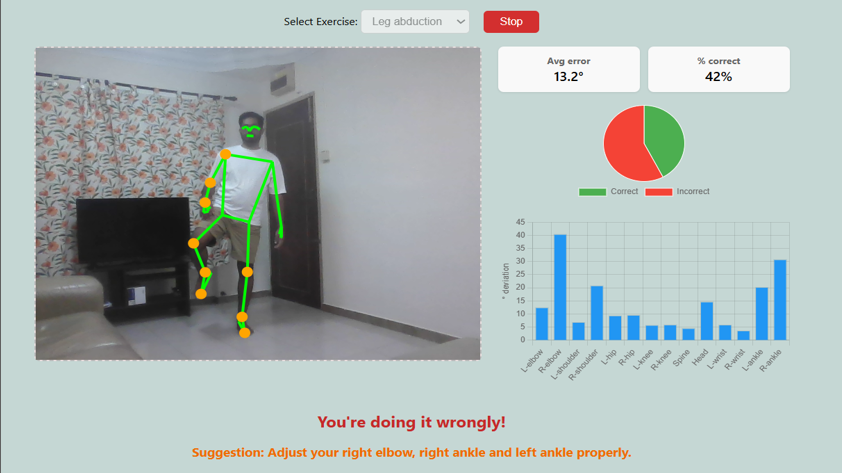
\includegraphics[width=.48\linewidth]{figs/ex4_bad_form.png}
  \caption{\textbf{Ex4 Leg-abduction.}
           Correct lift vs.\ insufficient abduction range; Deviated angles highlighted and included in the warning}
  \label{fig:qual_ex4}
\end{figure}

\begin{figure}[H]
  \centering
  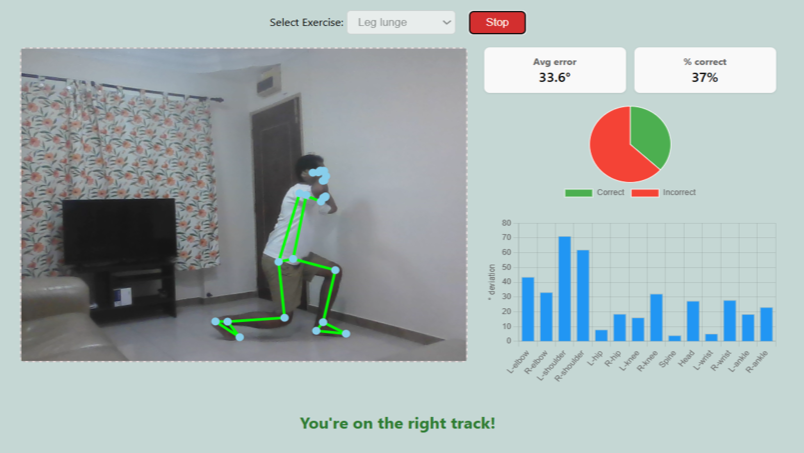
\includegraphics[width=.48\linewidth]{figs/ex5_correct.png}%
  \hfill
  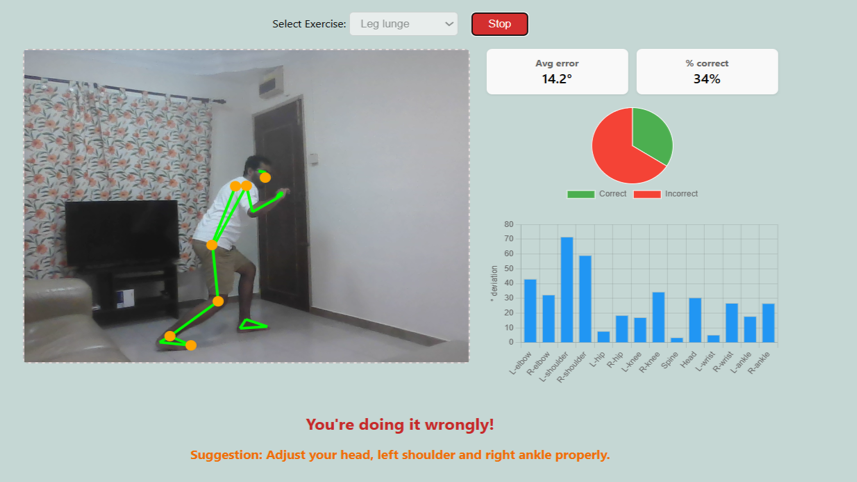
\includegraphics[width=.48\linewidth]{figs/ex5_bad_form.png}
  \caption{\textbf{Ex5 Lunge.}
           Correct vs.\ incorrect pose; Deviated angles highlighted and included in the warning}
  \label{fig:qual_ex5}
\end{figure}

\begin{figure}[H]
  \centering
  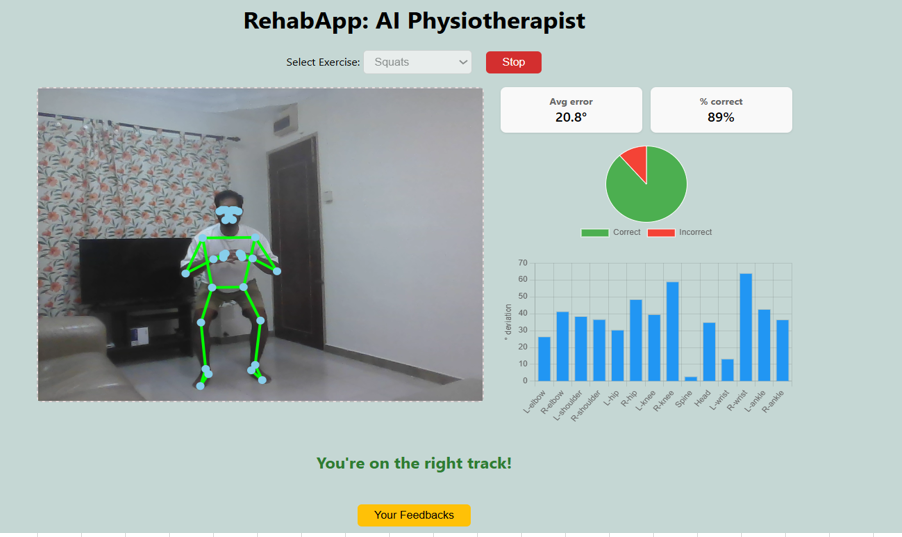
\includegraphics[width=.48\linewidth]{figs/ex6_correct.png}%
  \hfill
  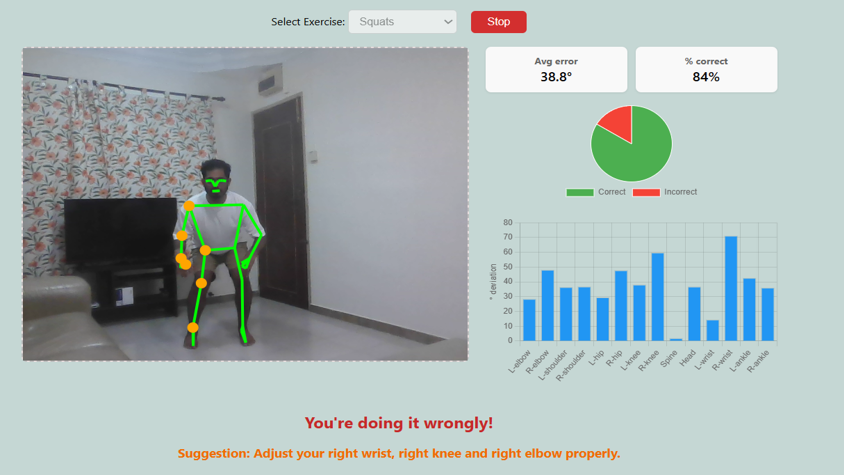
\includegraphics[width=.48\linewidth]{figs/ex6_bad_form.png}
  \caption{\textbf{Ex6 Squats.}
           Correct vs.\ incorrect pose; Deviated angles highlighted and included in the warning}
  \label{fig:qual_ex6}
\end{figure}

\begin{figure}[H]
  \centering
  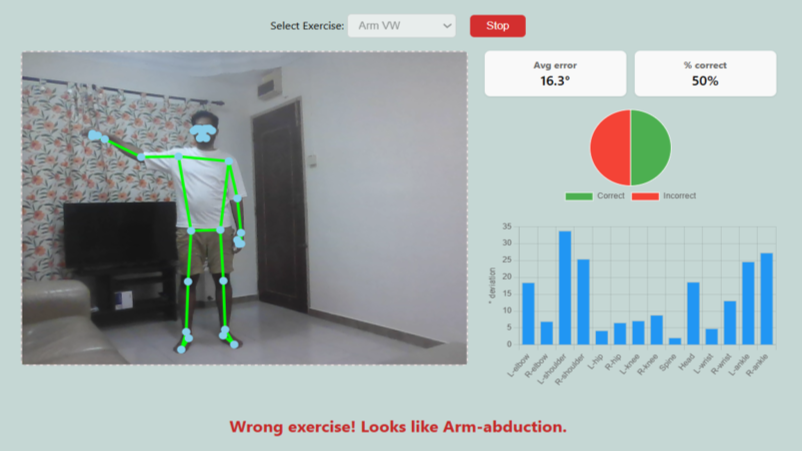
\includegraphics[width=.9\linewidth]{figs/wrong_exercise.png}
  \caption{\textbf{Wrong-exercise safeguard.}
           User selected \emph{Arm-VW} but performs a \emph{Arm-abduction}; system withholds joint advice and warns the user.}
  \label{fig:wrong_exercise}
\end{figure}

\begin{figure}[H]
  \centering
  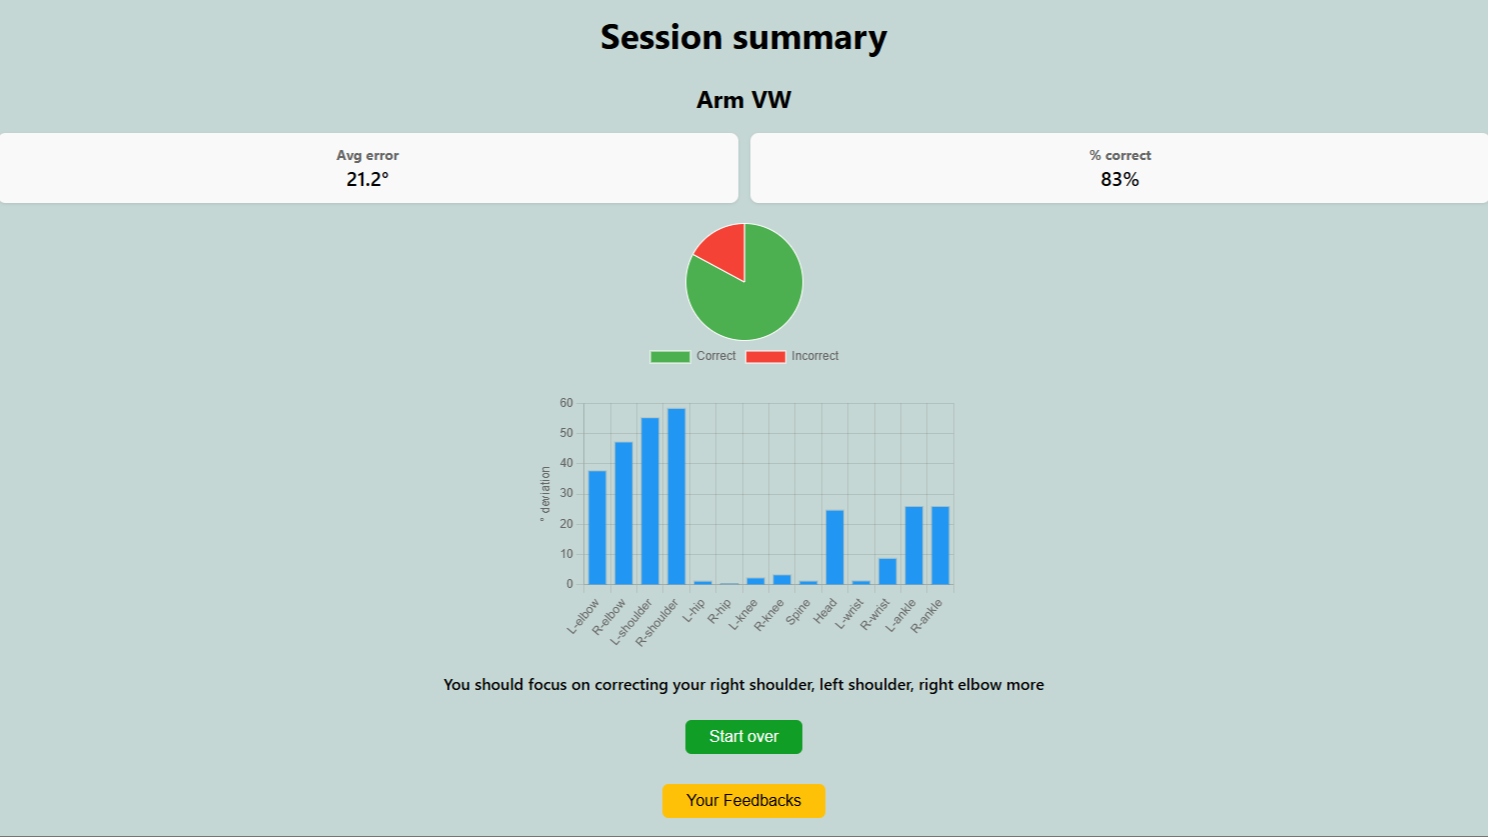
\includegraphics[width=.9\linewidth]{figs/summary_page.png}
  \caption{\textbf{End-of-session summary.}
           The pie chart, numeric tiles, and joint-error histogram from the session history, and an advice to guide the user on which joint angles need the most correction based on their overall session history}
  \label{fig:summary_page}
\end{figure}

% Ablation study
% --------
\subsection{Ablation study}
\label{sec:ablation}

To quantify how each architectural block contributes to the final
performance, we trained four variants of PoseQualityNetKP:

\begin{itemize}[leftmargin=1.5em]
  \item \textbf{A} – CNN feature extractor only  
  \item \textbf{B} – CNN + exercise–ID embedding  
  \item \textbf{C} – CNN + bidirectional LSTM (temporal encoder)  
  \item \textbf{FULL} – CNN + Bi-LSTM + exercise–ID embedding
\end{itemize}

Table~\ref{tab:ablate} reports the main metrics on the held-out test
split (\mbox{4112} windows).  All variants easily exceed real-time
throughput (FPS $\gg$ 30), but differ markedly in accuracy, regression
error, and model size.

% ---------
\begin{table}[H] 
  \caption{Ablation results on the REHAB24-6 test split.
           FPS measured with a 64-frame dummy clip on a single RTX 4090 (fp16).}
  \label{tab:ablate}
  \centering
  \small               % or \footnotesize to squeeze further
  \setlength{\tabcolsep}{3pt}   % tighten column spacing
  \begin{tabularx}{\columnwidth}{@{}lCCCCCCC@{}}
    \toprule
    \textbf{Variant} &
    \textbf{Rep-Acc} & \textbf{Rep-F1} &
    \textbf{Ex-Acc}  & \textbf{Ex-F1} &
    \textbf{MAE ($^{\circ}$)} & \textbf{FPS} & \textbf{Params (M)} \\ \midrule
    A (CNN)                 & 0.797 & 0.797 & 0.994 & 0.993 & 8.49 & 9\,160 & 0.25 \\
    B (CNN + Emb)           & 0.821 & 0.819 & 0.994 & 0.994 & 6.18 & 9\,126 & 0.25 \\
    C (CNN + Bi-LSTM)       & 0.853 & 0.853 & 0.996 & 0.996 & 6.12 & 7\,256 & 3.40 \\
    \textbf{FULL}           & \textbf{0.903} & \textbf{0.903} &
                              \textbf{0.997} & \textbf{0.997} &
                              \textbf{3.86} & 7\,383 & 3.41 \\
    \bottomrule
  \end{tabularx}
\end{table}
% ---------

\subsubsection{Key findings.}
\begin{enumerate}[leftmargin=1.35em,itemsep=2pt]
  \item \textbf{Exercise embedding (\textit{A} $\rightarrow$ \textit{B}).}
        Conditioning the quality and error heads on a one-hot exercise
        context yields an immediate boost in repetition accuracy
        (+2.4 pp) and cuts the MAE by \(\approx\,27\%\) at \emph{no}
        parameter cost, confirming that task-specific priors simplify
        the decision boundary.
  \item \textbf{Temporal encoder (\textit{A} $\rightarrow$ \textit{C}).}
        Replacing frame-wise pooling with a Bi-LSTM improves all four
        recognition metrics, most notably repetition quality
        (+5.6 pp).
  \item \textbf{Synergy (\textit{C} $\rightarrow$ \textit{FULL}).}
        Combining both blocks is \emph{additive}: the MAE is nearly
        halved relative to the CNN baseline (–4.6$^{\circ}$), while
        repetition accuracy gains a further +5 pp.  The parameter
        increase from 0.25 M to 3.4 M is marginal for modern GPUs and
        remains well within mobile budgets.
\end{enumerate}

Overall, the results validate the design choice of coupling a
light-weight temporal encoder with an exercise-aware context vector:
together they deliver the largest accuracy gains and the lowest
joint-angle error while maintaining real-time speed.


% Discussion and limitations
% --------
\subsection{Discussion and limitations}
\label{sec:limit}
% ---------------------------------------------------------------------------
\textbf{Model strengths.}  
PoseQualityNet-KP achieves convincing performance with a footprint of
only 3.4 M weights.  Its multi-head design yields three practical
advantages:  
(i)~joint-level feedback instead of a binary verdict,  
(ii)~automatic suppression of advice when the wrong drill is performed,
and  
(iii)~edge-ready inference (\(\sim\)30 fps on CPU, 7.5 k windows s\(^{-1}\)
in isolation).

\textbf{Residual failure modes.}  
Qualitative inspection reveals four recurring sources of error:
\begin{enumerate}[label=(\alph*),leftmargin=1.6em,itemsep=3pt]
  \item \emph{Self-occlusion.}  Exercises that hide an entire limb
        (e.g.\ seated squats with arms on thighs) occasionally produce
        invalid landmark estimates, which in turn mis-trigger the
        quality classifier.
  \item \emph{Camera pose.}  MediaPipe accuracy degrades once the sensor
        is pitched by more than \(\pm20^{\circ}\) or rolled
        non-horizontally, leading to spurious angle errors.
  \item \emph{Limited demographics.}  REHAB24-6 contains ten healthy
        young adults; performance on elderly or post-operative patients
        is untested.  Domain shift due to loose clothing, larger body
        mass, or assistive devices remains an open question.
\end{enumerate}

\textbf{Mitigation strategies.}  
Multi-view capture or synthetic occlusion augmentation could harden the
network against self-occlusion.  A fast entropy filter on the landmark
heatmaps would allow dynamic confidence weighting when the camera is
improperly oriented.  Finally, collecting a more diverse cohort and
fine-tuning the ankle channels with higher-resolution crops are expected
to close the remaining accuracy gap.

% Conclusions and future work
% --------
\section{CONCLUSIONS AND FUTURE WORK}
\label{sec:concl}
% ---------------------------------------------
We introduced PoseQualityNet-KP, a 3-head CNN–BiLSTM that turns a single
web-camera stream into joint-specific rehabilitation feedback.  Trained
on the cleaned REHAB24-6 corpus, the model reaches
\textbf{91.5\%} repetition-quality accuracy
(\(F_{1}=0.915\)), \textbf{99.5\%} \(F_{1}\) for exercise recognition,
and a \textbf{4.73\(^{\circ}\)} global MAE across 14 joint angles while
running fully on-device at real-time speed.  An ablation study confirms
that both the Bi-LSTM temporal encoder and the exercise-ID embedding are
essential: together they halve the angular error and raise quality
\(F_{1}\) by +10 pp with only a minor increase in parameters.

\textbf{Next steps} will address three axes:
\begin{enumerate}[label=\arabic*.,leftmargin=1.35em,itemsep=3pt]
  \item \emph{Robustness.}  Integrate a lightweight self-supervised
        pre-text task to improve landmark reliability under occlusion
        and extreme camera angles, and explore multi-view fusion when a
        second device is available.
  \item \emph{Personalisation.}  Add a 30-s calibration routine that
        learns user-specific joint-angle baselines and dynamically
        tightens tolerances as rehabilitation progresses.
  \item \emph{Deployment.}  Convert the network to 4-bit QAT ONNX,
        bundle it inside a cross-platform mobile SDK, and conduct a
        six-week field study with post-operative patients to quantify
        adherence and recovery gains versus usual care.
\end{enumerate}

Taken together, these extensions aim to transform the current prototype
into a clinically validated, low-cost companion for at-home
physiotherapy.

% Author contributions
% --------

\section{AUTHOR CONTRIBUTIONS}
The sole author, \textbf{Jithin Krishnan}, conceived the project idea, designed the methodology, implemented the system (including data processing, model development, and front-/back-end integration), performed all experiments, analysed the results, and wrote the manuscript.

% Author Referneces
% --------
\bibliographystyle{IEEEbib}
\bibliography{REFERENCES}

\end{document}
